% !TEX root = Master.tex

The procedure is continued also for key category cluster 8 with the same conditions, since we have similar issues as in the previous two clusters.
\\

Maximum likelihood estimation return parameters $\hat{\mu} = 7.21$, $\hat{\sigma} = 0.27$ and $\hat{\nu} = 0.46$ of the log-sales of \ac{KCC} 8 fitted to an ex-Gaussian distribution with no regressors.
\autoref{fig:kcc_8_margin} summarizes the findings in a histogram with an ex-Gaussian density curve with respect to the estimated parameters (\autoref{fig:kcc_8_density}) as well as the corresponding QQ-plot, where the points approximate the diagonal line (\autoref{fig:kcc_8_qqplot}). Normality of the residuals can be assumed, as the Shapiro-Wilk test returns a p-value of 0.99 and thus fails to reject the null hypothesis of non-normality. A histogram of the residuals and their density curve are shown in \autoref{fig:res_kcc_8_no_covariates}.
\\


%
%\begin{table}[H]
%\setlength\arrayrulewidth{1pt}  
%\centering
%\begin{adjustbox}{max width=\textwidth}\
%\begin{tabular}{|c|c|c|}
%\hline
%\rowcolor{lightgray} 
%$\hat{\mu}$ & $\hat{\sigma}$ & $\hat{\nu}$ \\ \hline
%7.21        & 0.27           & 0.46        \\ \hline
%\end{tabular}
%\end{adjustbox}
%\caption{Estimated parameters for log-sales of KCC 8 fitted to ex-Gaussian distribution with no covariate effects}
%\label{tab:estimated_parameters_kcc_8_no_covariates}
%\end{table}



 \begin{figure}[H]
\centering
\begin{subfigure}{.45\textwidth}
  \centering
  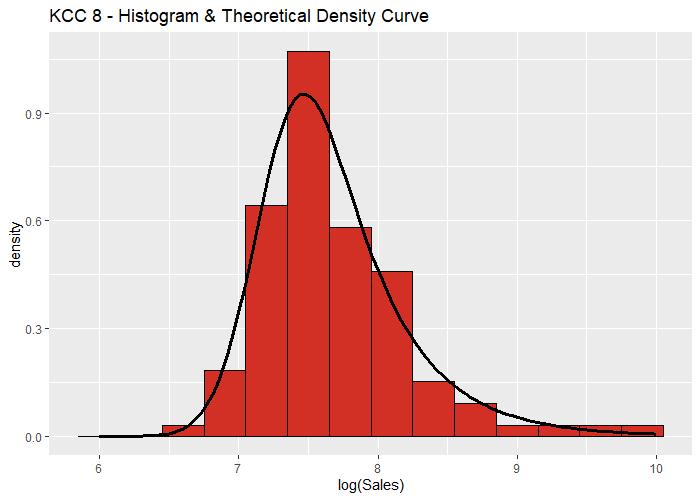
\includegraphics[width=\linewidth]{figures/kcc_8_density.png}
  \caption{Histogram \& theoretical density}
  \label{fig:kcc_8_density}
\end{subfigure}
\begin{subfigure}{.45\textwidth}
  \centering
  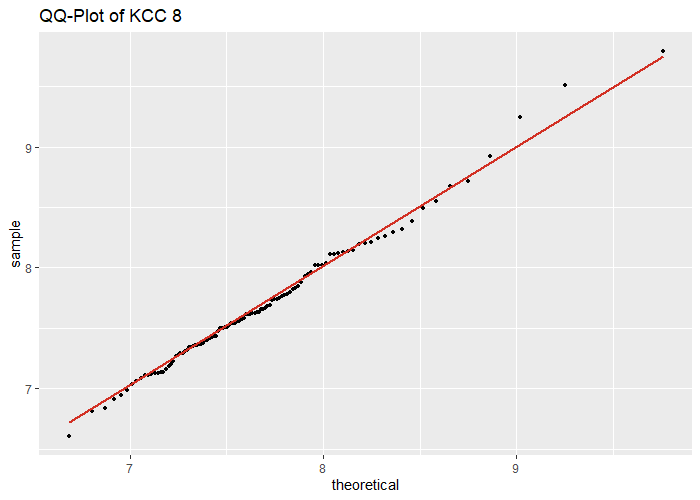
\includegraphics[width=\linewidth]{figures/kcc_8_qqplot.png}
  \caption{QQ-plot}
  \label{fig:kcc_8_qqplot}
\end{subfigure}
\caption{ex-Gaussian distribution fitted to log-sales of \ac{KCC} 8}
\label{fig:kcc_8_margin}
\end{figure} 


\begin{figure}[H]
\centering
  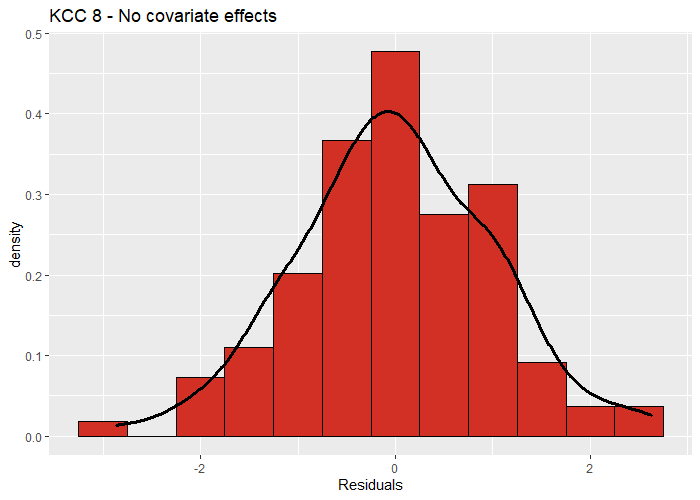
\includegraphics[width=0.45\linewidth]{figures/res_kcc_8_no_covariates.png}
  \caption{Residuals of KCC 8 log-sales fitted to an ex-Gaussian distribution with no covariate effects together with their density curve}
  \label{fig:res_kcc_8_no_covariates}
\end{figure}




Again, Model \ref{eq:gamlss_kcc_2} is applied to the log-sales. The summary output and estimated parameters with confidence intervals can be seen in \autoref{fig:gamlss_kcc_8_estimated_parameters} and in \autoref{tab:nu_ci_kcc_8}. We notice that models fit is acceptable matching the elevated sales during promo weeks and that the variability is strictly decreasing with the overall range having a range between 0.1 and 0.3. Skewness remains low in the data.
\\




%\VerbatimInput[frame = single, label = "GAMLSS Fit on KCC 8" ]{gamlss_fit_kcc_8_try1.txt}


\begin{table}[H]
\centering
\begin{tabular}{l|c|c|c|l}
  \hline
  \rowcolor{white}
 \textbf{$\hat{\mu}$ Coefficients} & \textbf{Estimate} & \textbf{Std. Error} & \textbf{t value} & \textbf{p-value} \\ 
  \hline\hline
\textit{$\beta_{01}$ (Intercept)} & 5.51 & 0.17 & 31.56 & 0.00 *** \\ 
  \textit{$f_{11}$(time)} & 0.00 & 0.00 & 5.06 & 0.00 *** \\ 
  \textit{$f_{12}$(total\_markdown\_pct)} & 4.53 & 0.45 & 10.02 & 0.00 *** \\ 
  \textit{promo\_typeBlack Friday} & -0.65 & 0.37 & -1.75 & 0.08  \\ 
  \textit{promo\_typeFriends \& Family} & -0.04 & 0.66 & -0.55 & 0.96 \\ 
  \textit{promo\_typeBlack Friday:total\_markdown\_pct} & 0.88 & 0.73 & 1.20 & 0.23  \\ 
  \textit{promo\_typeFriends \& Family:total\_markdown\_pct} & -0.76 & 1.24 & -0.62 & 0.54  \\ \hline
\end{tabular}
\caption{Estimated coefficients of \ac{GAMLSS} fit on log-sales of \ac{KCC} 8}
\label{tab:gamlss_coeff_kcc_8}
\end{table}






\begin{figure}[H]
\centering
  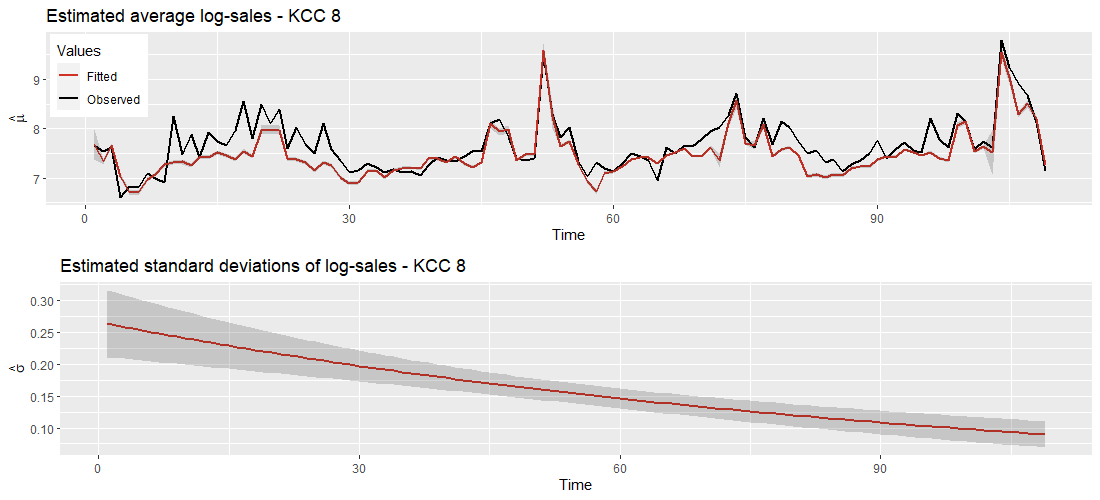
\includegraphics[width=0.95\linewidth]{figures/gamlss_kcc_8_estimated_parameters.png}
  \caption{Estimated location parameter $\hat{\mu}$ compared to the observed values and scale parameter $\hat{\sigma}$ with confidence bands of GAMLSS fit - KCC 8}
  \label{fig:gamlss_kcc_8_estimated_parameters}
\end{figure}



\begin{table}[H]
\setlength\arrayrulewidth{1pt}  
\centering
\begin{adjustbox}{max width=\textwidth}\
\begin{tabular}{c|c|c}
\hline
\rowcolor{white} 
\textbf{Lower} & $\hat{\nu}$ & \textbf{Upper} \\ \hline\hline
0.181        & 0.158           & 0.203        \\ \hline
\end{tabular}
\end{adjustbox}
\caption{Estimated skewness parameter $\hat{\nu}$ of GAMLSS fit with 95\% confidence interval bounds - KCC 8}
\label{tab:nu_ci_kcc_8}
\end{table}



Time as well as the total markdown percentage exhibit similar positive effects on the response as in \ac{KCC} 6, collapsing into a straight line. The promo effects seem to be more balanced, with different interquartile ranges for all cases.
\\


\begin{figure}[H]
\centering
  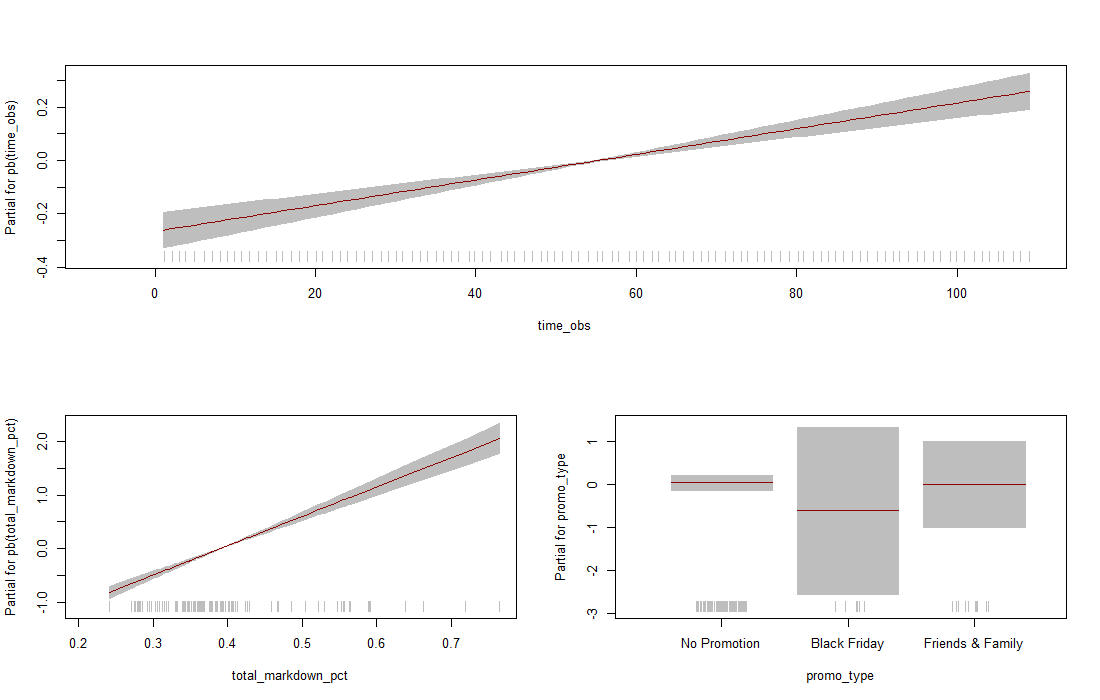
\includegraphics[width=0.95\linewidth]{figures/gamlss_effects_kcc_8.png}
  \caption{Covariate effects on the expected response variable (log-sales) of GAMLSS fit - KCC 8}
  \label{fig:gamlss_effects_kcc_8}
\end{figure}



Looking at \autoref{fig:gamlss_residuals_kcc_8} and \autoref{tab:gamlss_residuals_kcc_8} for the distribution of the quantile residuals, the fitting method for this cluster is also justified. The Shapiro-Wilk test is "weaker" in comparison to the fit without covariate effects with a p-value of 0.86, which is still a solid reason to retail the null hypothesis of normality.


\begin{figure}[H]
\centering
  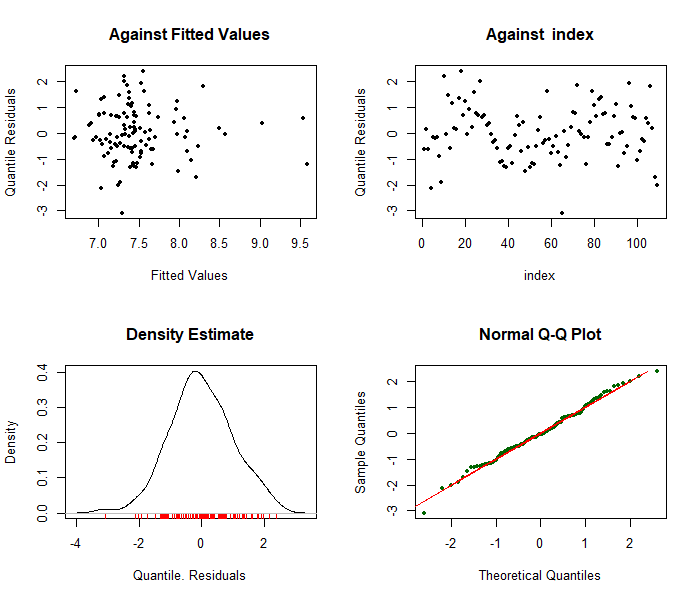
\includegraphics[width=0.95\linewidth]{figures/gamlss_residuals_kcc_8.png}
  \caption{Residuals of GAMLSS fit - KCC 8}
  \label{fig:gamlss_residuals_kcc_8}
\end{figure}


%\VerbatimInput[frame = single, label = "Residuals of GAMLSS Fit on KCC 8" ]{gamlss_residuals_kcc_8.txt}


\begin{table}[H]
\centering
\begin{tabular}{c}
\hline
\rowcolor{white} 
\textbf{Summary of the Quantile Residuals} \\ \hline\hline
 $\begin{array}[t]{ r @{{}={}} l }
\text{mean} & 0.0004673878                          \\ 
\text{variance} & 1.008849                          \\ 
\text{coef. of skewness} & -0.02817569              \\ 
\text{coef. of kurtosis} & 3.04467                 \\ \hline
\end{array}$
\end{tabular}
\caption{Residuals of GAMLSS Fit on KCC 8}
\label{tab:gamlss_residuals_kcc_8}
\end{table}



%\inputRoutput[caption={Residuals of GAMLSS Fit on KCC 8},numbers=left,numberstyle=\tiny, label=output:gamlss_residuals_kcc_8]{gamlss_residuals_kcc_8.txt}


